%*******************************************************************************
% Copyright (c) 2014 Formal Mind GmbH and others
% All rights reserved. This program and the accompanying materials
% are made available under the terms of the Eclipse Public License v1.0
% which accompanies this distribution, and is available at
% http://www.eclipse.org/legal/epl-v10.html
% 
% Contributors:
%     Michael Jastram - initial Copy
%     Maha Jastram - susequent improvements
%******************************************************************************/

% ===================================================================================
\section{Basic Concepts}
\index{Concepts}
% ===================================================================================

In this tutorial, we will use the ReqIF terminology, which can be confusing.  Therefore, please familiarize yourself with the terminology first (Section~\ref{sec:terminology}.

\begin{warning}
In ReqIF terminology, a requirement is called \term{SpecObject}, a link is a \term{SpecRelation}, and the document view consists of \term{SpecHierarchies}.  Confused? Then please take the time to at least glance over Section~\ref{sec:terminology}.
\end{warning}

% ===================================================================================
\section{Tutorial 1: Creating a basic ReqIF Model}
% ===================================================================================

In this Section, we will build a ReqIF model from scratch, step by step.

% -----------------------------------------------------------------------------------
\subsection{Install \pror{}}
% -----------------------------------------------------------------------------------

The easiest way for installing \pror{} is downloading \href{http://formalmind.com/studio}{formalmind Stu\-dio}.  This is a standalone-application that is based on Eclipse ProR, combined with some enhancements.

 Alternatively, you can install ProR in any Eclipse-Installation via its update site (listed on the \href{https://www.eclipse.org/rmf/download.php}{RMF Download page}).  This is recommended for advanced users only who need to integrate RMF with other Eclipse-based components.

\begin{info}
The installation is described in detail in Section~\ref{sec:installation}.
\end{info}

% -----------------------------------------------------------------------------------
\subsection{Create the Model}
% -----------------------------------------------------------------------------------

\begin{itemize}

\item
  If you do not already have one, create a new project: Select  \menu{File | New | Project};
\item
  Select \menu{File | New | Reqif10 Model};
\item
  Select the project and name the file tutorial.reqif.  Click \menu{Finish};
\item
  In the Window named ``tutorial.reqif'', double-click on ``Requirements
  Document'' button in the ``Specifications'' panel.
\end{itemize}

After this, your window should look more or less as follows:

\begin{figure}[H]
  \centering
  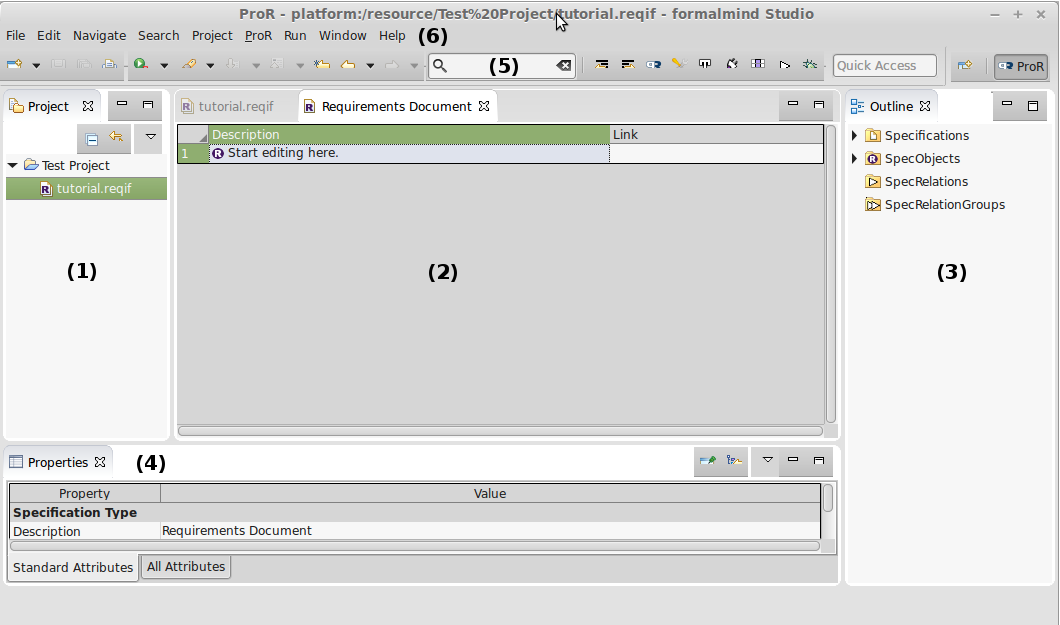
\includegraphics[width=\linewidth]{../rmf-images/Screenshot_intro.png}
  \caption{The \pror{} user interface}
\end{figure}

You will see your ReqIF file in the Project Explorer window (1).

The Editor (2) shows your Specifications.

In the Editor, you see the SpecObjects that exist in this Specification.  There is currently only one, with the description ``Start editing here''.

The Outline (3) has four folders:
\index{outline view}

\begin{description}
\item[Specifications] shows the Specifications in the ReqIF.  You can expand the tree to expose the hierarchy of SpecObjects in the ReqIF model.
\item[SpecObjects] shows all SpecObjects in the ReqIF model as a flat list.  Keep in mind that SpecObjects in Specifications are references.  In contrast, this folder shows all SpecObjects created for the ReqIF model, whether or not they are referenced.
\item[SpecRelations] shows all SpecRelations in the ReqIF as a flat list.  For now, we will ignore SpecRelations.
\item[SpecRelationsGroups] are special constructs to can be used for grouping SpecRelations with the same source and target.
\end{description}

The properties of a selected Element are shown in the Properties view (4).  As the only Requirement in the model is selected, we see its SpecObjectType (``Requirements Type'') and its only Attribute (``Description'') with the value ``Start editing here.''.  There are two tabs ``Standard Attributes'' and ``All Attributes'' at the bottom of the Properties view.  The ``Standard Attributes'' tab shows you all standard attributes of the selected element.  The ``All Attributes'' shows all existing ReqIF attributes of the selected element.

Above the main working windows it the tool bar (5) and, at the very top, the menu bar (6).

% -----------------------------------------------------------------------------------
\subsection{Customizing the SpecType}
% -----------------------------------------------------------------------------------

To get familiar with the system, we will:

\begin{itemize}
\item
  Add two more attributes to the SpecObjectType called ``ID'' and ``Owner'' and
\item
  We will show those Attributes in the Specification
\end{itemize}

To add new attributes, we open the Datatype Configuration dialog with \menu{ProR | Datatype Configuration}.  Alternatively you can also click on 
\includegraphics[height=0.8em]{../rmf-images/icons/full/obj16/SpecType.png} in the Tool Bar.

The resulting dialog box has two folders in the upper pane: one for SpecTypes and one for Datatypes.  Currently, there is only one Datatype (T\_String32k) and two SpecTypes, one called ``Requirements Type'' with one attribute ``Description'' and one called ``Specification Type'' with one attribute ``Description''.

In the lower pane are the details in regards to each attribute.

We add more Attributes to ``Requirements Type'' by right-clicking ``Requirements Type'' and selecting \menu{New Child | Attribute Definition String}.  This will create a new element.  Upon selecting, we can rename it and tailor the details.  Double-click on the ``Long Name'' variable and type in ``ID''.  Change the Type by double-clicking the field and choosing ``T\_String32k'' from the drop-down menu.  Repeat the process but this time change the ``Long Name'' to ``Owner''.  In the end, the dialog should look as follows

\begin{figure}[H]
\centering
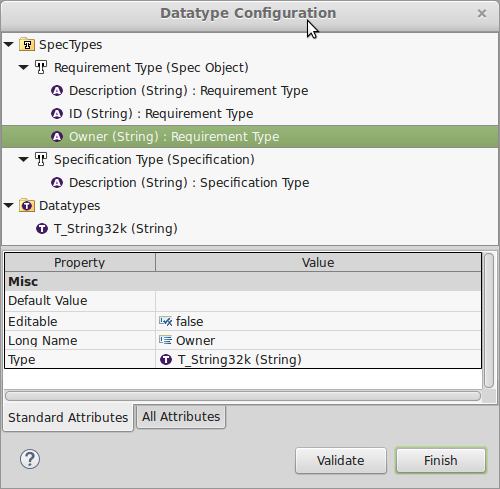
\includegraphics[width=0.8\linewidth]{../rmf-images/datatype.png}
\caption{Datatype Configuration Dialog}
\label{fig:datatype_configuration}
\end{figure}

Upon closing the dialog, little will have changed - the Specification still shows just two columns, Description and Link.  However, if you select the requirement, you will see the new Properties (ID and Owner) in the Property view.

% -----------------------------------------------------------------------------------
\subsection{Showing the new Attributes in the Specification}
% -----------------------------------------------------------------------------------

To show the new Attributes in the Specification, we have to configure the Specification columns.  We do this by selecting \menu{ProR | Column Configuration}.  You can also click on the spreadsheet icon in the Tool Bar.

The resulting Dialog shows one entry, ``Description'' for the one and only Column of the Specification.  In the ``Value'' column double click on ``Description to choose it and replace it with ``ID''.

By clicking on the ``Add Column'' icon at the top of the dialog, create a new column and name it ``Description''.  In this view, the columns can be dragged and dropped to change their order as desired.

The resulting window should look like this:

\begin{figure}[H]
\centering      
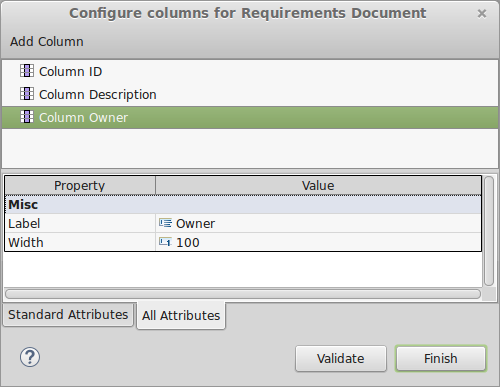
\includegraphics[width=0.8\linewidth]{../rmf-images/columnconfig.png}      
\caption{Column Configuration}
\label{fig:column_configuration}
\end{figure}

Note that you have to provide free text for the columns for the same reason that we used free text for the ``Labels'' earlier: This way we can easily match multiple SpecObjects of different types.

You can actually adjust the width of the columns simply by dragging the column headers.

% -----------------------------------------------------------------------------------
\subsection{Adding new SpecObjects}
% -----------------------------------------------------------------------------------

Now we can finally add SpecObjects by right-clicking on a row in the Specification.  In the context-menu, there are two submenus: ``New Child'' and ``New Sibling''.  ``New Child'' is the only way to produce a hierarchical structure.

In both menus, there are three entries ``Spec Hierarchy'', ``Adding SpecObjects'' and ``SpecObject (Requirement Type)''.  Some background is needed here:

We said before that Specifications contain references to SpecObjects.  A SpecHierarchy is the ``Wrapper'' that allows the hierarchical structure and that points to the referred SpecObject.  Usually, we don't have to be concerned with them.  Therefore the second option: If selected, a new SpecHierarchy is created and associated with a new SpecObject, which in turn is set immediately to the given SpecObjectType.  If we had more than just one SpecObjectType (besides ``Requirements Type''), there would be an entry for each type in the context menu.

To continue the exercise, select the child ``SpecObject (Requirement Type)''.  Now we have two SpecObjects.  The original is numbered on the far left-hand side of the pane with a 1.  The second one, the child, is numbered 1.1.  Now we should change the ID's of each entry.  Click in the ``ID`` for number 1 and type in INF-1.  Under Description, type ''A ProR tutorial``.  For the second, change the ID to REQ-1 and ''Learn now to create a new requirement'' in the Description column.

Feel free to add a few more rows and or even new structures.  Yours should look somethinig similar to this:

\begin{figure}[H]
\centering
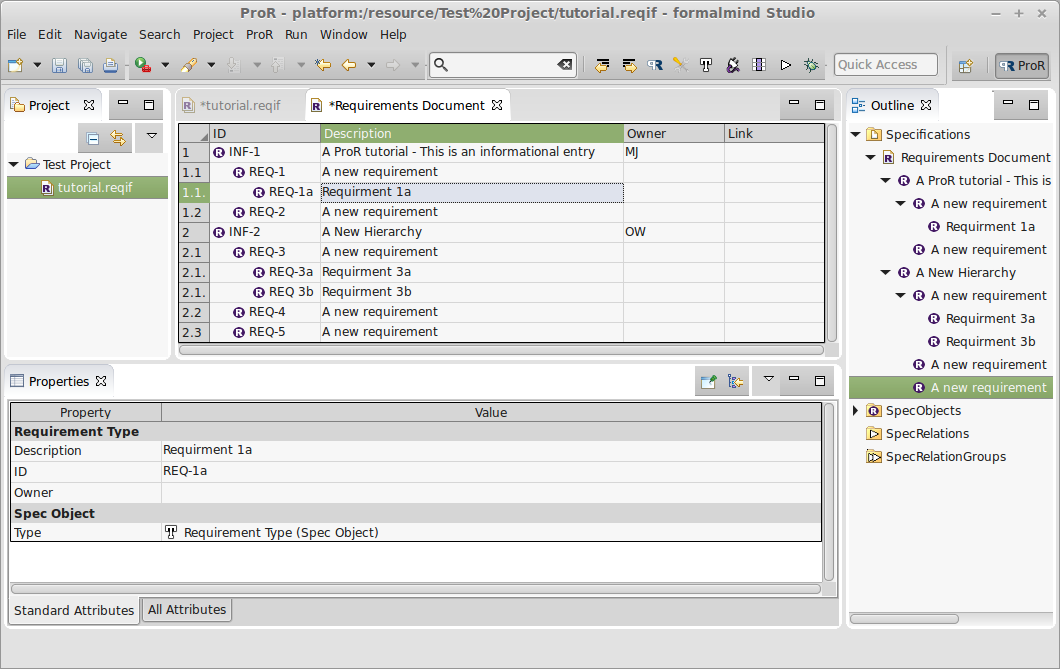
\includegraphics[width=\linewidth]{../rmf-images/hierarchy_example.png}      
\caption{Adding SpecObjects}      
\label{fig:Requirements Hierarchy}
\end{figure}

\begin{figure}[H]
\centering
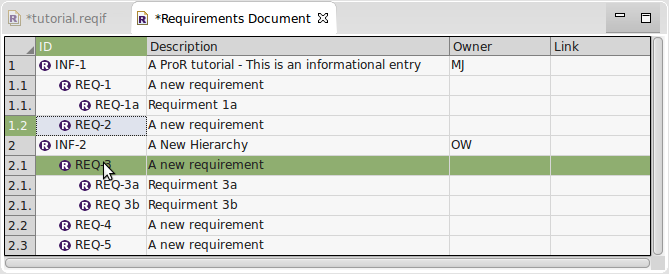
\includegraphics[width=\linewidth]{../rmf-images/draganddrop.png}    
\caption{Drag and Drop}      
\label{fig:dragAndDropChild}
\end{figure}
You can drag and drop a SpecObject as a sibling or a child.  The highlighting feedback will enable you to see what you're moving and where to.  For instance, if you are dragging a SpecObject over another one, the entire cell will be highlighted.  This means, that the SpecObject will be assigned as a child to the dropped SpecObject.

If you are dragging a SpecObject between two rows, you also get visual feedback on whether the SpecObject will be assigned as a sibling.

After some playing around, our Specification may look somewhat like this:

\begin{figure}[H]
\centering      
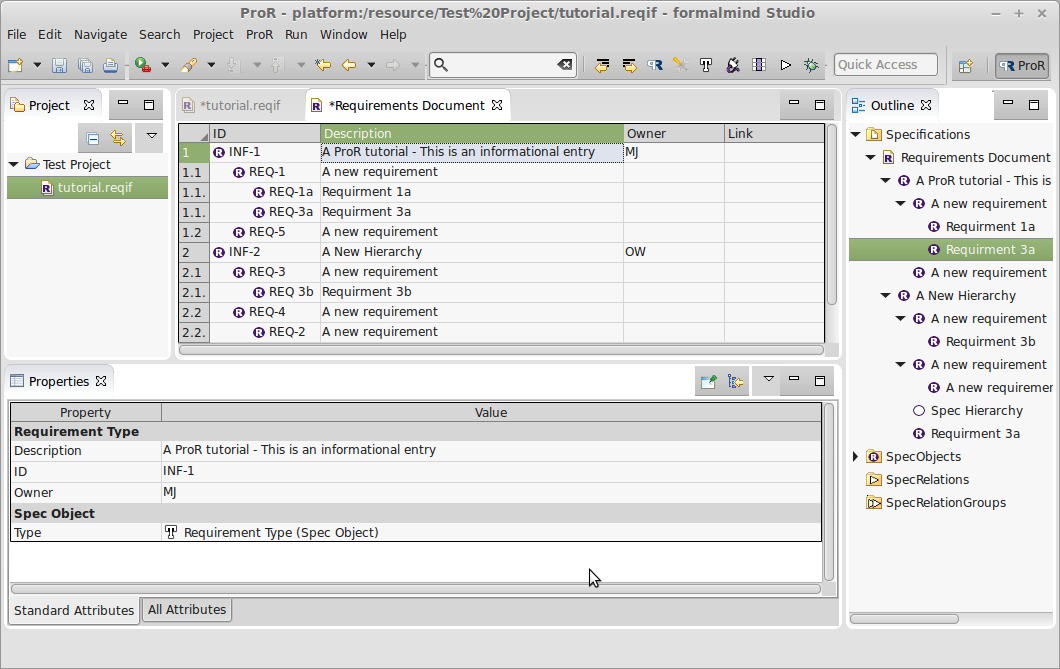
\includegraphics[width=\linewidth]{../rmf-images/hierarchy_dad.png}      
\caption{Improved Specification}      
\label{fig:improvedSpec}
\end{figure}

% -----------------------------------------------------------------------------------
\subsection{Export Specification as HTML}
% -----------------------------------------------------------------------------------

If you want to export your Specification as HTML, go to File \textgreater{} Export as HTML.  The HTML representation is generated and saved into your target folder.

% -----------------------------------------------------------------------------------
\subsection{Conclusion}
% -----------------------------------------------------------------------------------

Quite an achievement—but there's still a bit of a way to go.  One improvement we can make is simplifying data entry.  Another is improving  the visibility of the descriptions.  In the next part of the tutorial, we will address these issues.

% ===================================================================================
\section{Tutorial 2: Use Presentations}
% ===================================================================================

We will continue where we left off at the end of Tutorial 1 and we will assume that you have \pror{} open with a model identical or similar to the one we created earlier.

In this tutorial we will introduce Presentations.  Presentations are Eclipse Plug-Ins that extend the functionality of \pror{}.  Specifically:

\begin{itemize}
\item
  Presentations can change the way Attributes are rendered in the Specification,
\item
  Presentations can change the way Attributes are edited in the Specification and
\item
  Presentations can perform tasks in the background.
\end{itemize}

\pror{} comes with a number of standard presentations that we will introduce in this tutorial.

% -----------------------------------------------------------------------------------
\subsection{Linewrap Presentation}
% -----------------------------------------------------------------------------------

By default, text is not wrapped in cells.  We will enable the Linewrap Presentation for the Description column.

To do this, we select, from the menu,  \pror{} \textgreater{} Presentation Configuration.  Alternatively you can click the power card in the tool bar.

The dialog box so far has no entries.  The drop-down menu, ``Select Action...'', at the top allows us to create new Presentations.  We select the ``Linewrap'' Presentation.  This will create a new entry in the upper pane.  Upon selecting it, we can configure it in the lower pane.

A Linewrap Presentation has only one configuration element, the Datatype.  We select ``T\_String32k''.  This means that from now on, all Attributes of this type will be rendered with the Linewrap Presentation.  Upon completion, the dialog should look like this:

\begin{figure}[H]
\centering
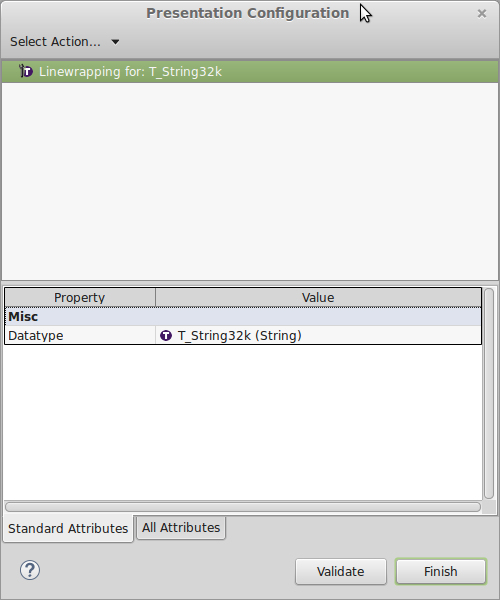
\includegraphics[width=0.8\linewidth]{../rmf-images/presentationconfig.png}      
\caption{Presentation Configuration Dialog Box}      
\label{fig:presentationConfig}
\end{figure}

Upon closing the dialog, the lines that are too long should be wrapped automatically.  Also, upon clicking on a cell, the content is now wrapped in the editor.

% -----------------------------------------------------------------------------------
\subsection{ID Presentation}
% -----------------------------------------------------------------------------------

It would be nice if every SpecObject had its own unique ID.  Actually, it does (it is shown in the Property View, if a SpecObject is selected in
the Outline View).  But that ID is meant for machines and is not practical.

The ID Presentation allows the automatic creation of more user-friendly IDs.  Let's create one.

Remember that Presentations are associated with Datatypes, not Attributes.  Thus, we first have to create a new Datatype called ``T\_ID``.  We then associate that Datatype with the Attribute ``ID''.  We described this process in the first tutorial.  Here is a screen-shot of the configuration dialog, when all is done:

\begin{figure}[H]
\centering      
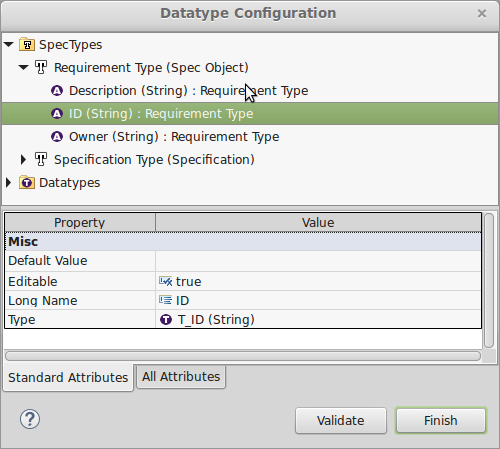
\includegraphics[width=0.8\linewidth]{../rmf-images/t_id.png}      
\caption{Datatype Configuration Dialog}      
\label{fig:datatypeConfig}
\end{figure}

The last step is, like before, to associate that Datatype with the Presentation.

We open the Presentation Configuration and create a new Presentation from the dropdown menu ``Select Action...'', this time of type ``Id'' Presentation.  We associate it with the newly created Datatype.  After configuration, ould look as follows:

\begin{figure}[H]
\centering      
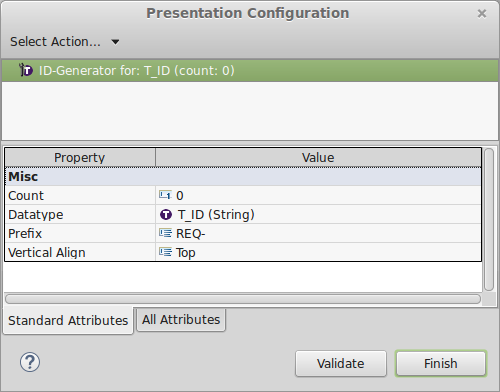
\includegraphics[width=0.8\linewidth]{../rmf-images/presentation_id.png}      
\caption{ID Configuration Detail}      
\label{fig:idConfig}
\end{figure}

Note that you could adjust the prefix, count and the vertical alignment of the presentation.

NOTE: At this point, the Presentation doesn't check yet for duplicates.  It simply grabs a new value from count, increments it and uses it.  Also, existing values are not overwritten.

% ===================================================================================
\section{Tutorial 3: Advanced SpecTypes}
% ===================================================================================

So far, we have a model with only one SpecObjectType.  In this tutorial, we will show how we can work with multiple SpecTypes, and we will introduce other SpecTypes.

% -----------------------------------------------------------------------------------
\subsection{Multiple SpecTypes}
% -----------------------------------------------------------------------------------

The first entry in our Specification (``A \pror{} Tutorial'') isn't really a requirement.  Thus, it doesn't need an ID or an owner, and it would be nice to Highlight it somehow.  For Highlighting, we have the Headline Presentation.  We will:

\begin{itemize}

\item
  Create a new ``Headline'' SpecObjectType
\item
  Create a new Datatype that will be used for the Headline content
\item
  Associate that Datatype with the Headline Presentation
\end{itemize}

With \pror{} \textgreater{} Datatype Configuration we get the Dialog where we can create new SpecTypes and Datatypes.  For the first time, we create a new SpecObjectType by right-clicking on ``SpecTypes''.  One of the entries in the child menu is ``SpecObject Type''.

Once created, we select it and rename to ``Headline Type'' it in the properties.

Then we give it a new Attribute called ``Description''.

NOTE: It is important that we call it description.  This matches the Attribute from ``Requirement Type''.  By using the same name, we ensure that the Attributes appear in the same column, even though they are different Attributes.

We do not set the type yet, as we need to create a new one.  We do this by right-clicking on ``Datatypes'' (or on the ''T`` in the tool bar.  Create a child under ``Datatypes'' and  ``Definition String''.  Call it ``T\_Headline'' and set the length to 50.  Now we can go back to the Description Attribute and set the type to T\_Headline.

When all this is done, the configuration should look like this:

\begin{figure}[H]
\centering      
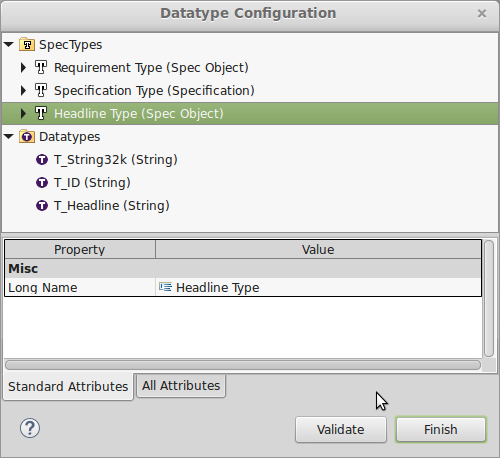
\includegraphics[width=0.8\linewidth]{../rmf-images/datatype_Headline_desc.png}      
\caption{Datatype Configuration for the Headline Presentation}      
\label{fig:headlineConfig}
\end{figure}

You can change the type of a SpecObject by selecting it and changing it in the Properties view.  Please note that currently all existing values are lost when changing the type.

After the changes, the GUI should look as follows:

\begin{figure}[H]
\centering      
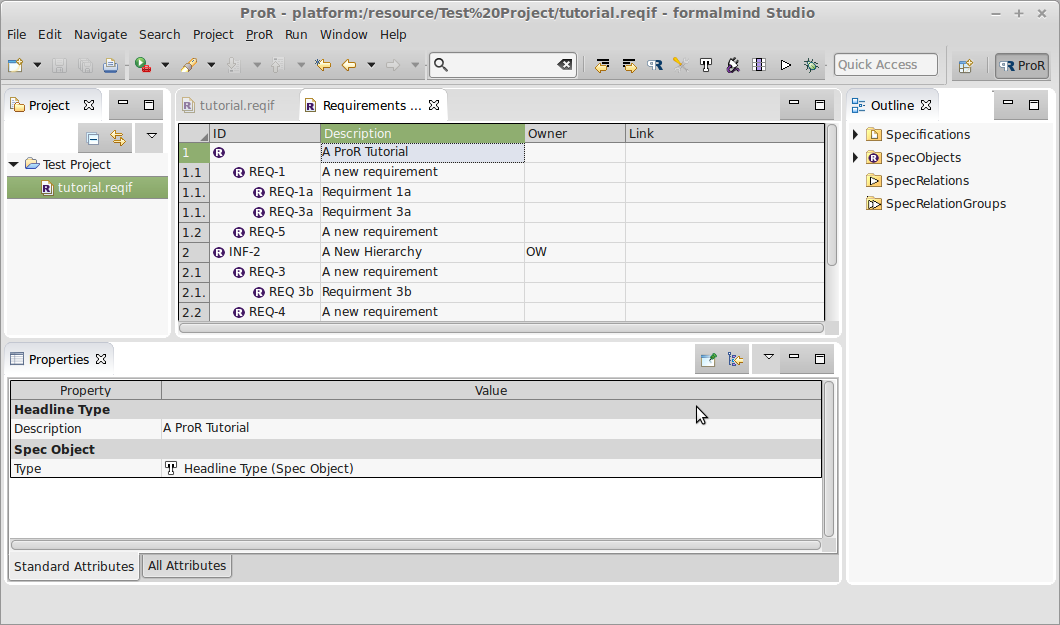
\includegraphics[width=\linewidth]{../rmf-images/desc_headline.png}      
\caption{Activated Headline Configuration}      
\label{fig:activeHeadlineConfig}
\end{figure}

Note the following:

\begin{itemize}
\item
  The columns ``ID'' and ``Owner'' are now empty and cannot be edited
\item
  Note how the Property View changes as you select SpecObjects of different types
\item
  Right-clicking on a row now shows one more option for child/sibling creation: A new entry of type ``Headline Type''
\end{itemize}

Last, we will use the Headline Presentation for the type T\_Headline.  This is done via the Presentation Configuration.  By the way, you can also change the font size of the headline in the ``Size'' attribute.  The result should look something like this:

\begin{figure}[H]
\centering      
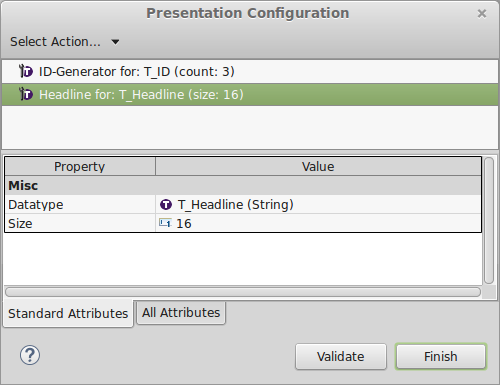
\includegraphics[width=0.8\linewidth]{../rmf-images/Presentation_headline.png}      
\caption{Presentation Configuration for Headline}      
\label{fig:headlineConfig2}
\end{figure}

% -----------------------------------------------------------------------------------
\subsection{Other SpecTypes}
% -----------------------------------------------------------------------------------

You may have noticed in the Datatype Configuration Dialog, that right-clicking on ``SpecTypes'' offered more options, besides ``SpecObject Type''.  A number of ReqIF-Elements can have Attributes.

We will now create a ``Specification Type'' and assign it to our Specification.

Try to create a ``Specification Type'' and configure it as shown in the screenshot:

\begin{figure}[H]
\centering      
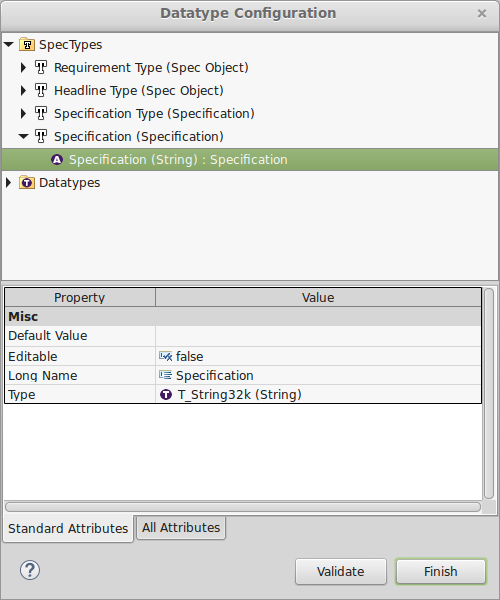
\includegraphics[width=0.8\linewidth]{../rmf-images/new_spectype.png}      
\caption{Creating a New SpecType}      
\label{fig:newSpecType}
\end{figure}

Next, we will assign this type to the one Specification that we have.  To do this we select the Specification in the Outline View.  That will show
the Specification's Properties in the Properties View.  The ``Type'' Property is empty.  We select ``Specification Type'' from the drop down.
As soon as it is selected, the Attribute ``Description'' will appear in the properties view.

% ===================================================================================
\section{Tutorial 4: Links (SpecRelations)}
% ===================================================================================

The implementation of SpecRelations is not complete yet.  Still here are a few pointers to show what is planned.

% -----------------------------------------------------------------------------------
\subsection{Creating SpecRelations}
% -----------------------------------------------------------------------------------

SpecRelations are created by ``Link-Dragging''.  This is platform specific:

\begin{itemize}

\item
  Linux: Dragging with Ctrl-Shift
\item
  Mac: Hold down OPTION and APPLE/COMMAND keys while dragging.
\item
  Windows: Dragging with Alt
\end{itemize}

Showing links as children can be switched on or off with the little triangle icon in the toolbar:

After creating a link:

\begin{itemize}
\item
  The ``Link'' column shows incoming and outgoing links
\item
  The SpecRelations are shown as children in the Specification view
\end{itemize}

SpecRelations can have their own Types.  Once a type is set, the corresponding columns in the Specification are rendered using Presentations, etc.  However.  the Type has to be set explicitly (a link created with dragging has currently no Type).

Here is a Screenshot of a Specification with some Links and a SpecRelationType that includes a ``Description'' Attribute:

\begin{figure}[H]      
\centering      
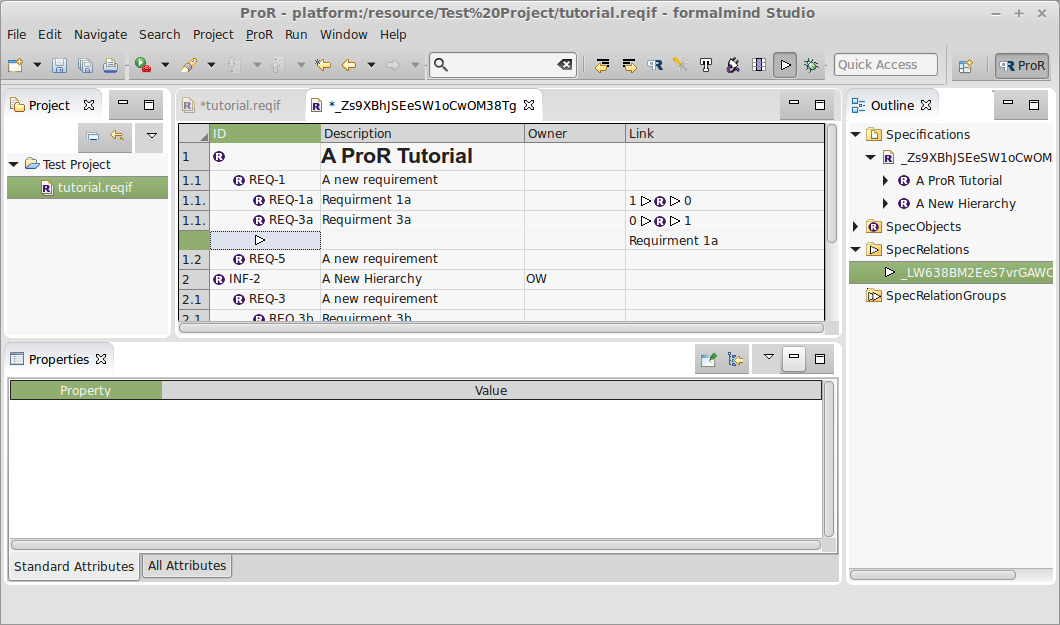
\includegraphics[width=\linewidth]{../rmf-images/links.png}      
\caption{Showing Links in the GUI}      
\label{fig:linksInGui}
\end{figure}

Note the following:

\begin{itemize}
\item
  The right column shows incoming and outgoing links
\item
  The number to the left of the triangle is incoming links, the other outgoing links
\item
  The outgoing link from REQ-1 is shown
\item
  The link from REQ-1 has a description, and it shows the destination name in the ``Link'' column
\end{itemize}

% -----------------------------------------------------------------------------------
\subsection{Outline View}
% -----------------------------------------------------------------------------------

Note that the Outline shows a folder with all SpecRelations.

